\subsubsection{Grid} \label{GridSection}

The truncated domain is discretised as a grid, with a structured Cartesian format used to reduce solver complexity. Additionally, the dimensions and resolution of the domain were set to $2 \ \mathrm{m}$ x $2 \ \mathrm{m}$ and $300$ x $300$ grid points (where $\Delta x = \Delta y$), which equates to $90,000$ total grid points. In the grand scheme of CAA solvers this is relatively small, however the goal is simply to explore and optimise the parameters (on a lab PC using non-parallelised code) rather than investigate actual representative geometry. Should this be applied to a real problem, one might expect a simulation to reach into the tens of millions of grid points with fully parallelised code running on a HPC research cluster. 

To calculate a maximum PML-induced error within the Euler domain, a reference domain $\mathrm{mult}_{x}$ larger than the Euler domain is instanced. The reference domain also includes a PML of substantial width and damping, located far enough away from the mapped Euler location so that the initial pulse does not reach the boundaries during the total computation time. This avoids incurring any errors that might skew the 'reference' nature of the larger domain. The location of the Euler domain is mapped to the reference domain and numerically solved field variables from both solutions are compared to determine a PML-induced error. An illustration of which can be seen in Figure \ref{fig:REFPMLDomain}.

\begin{figure}[h!]
\centering
\makebox[0pt]{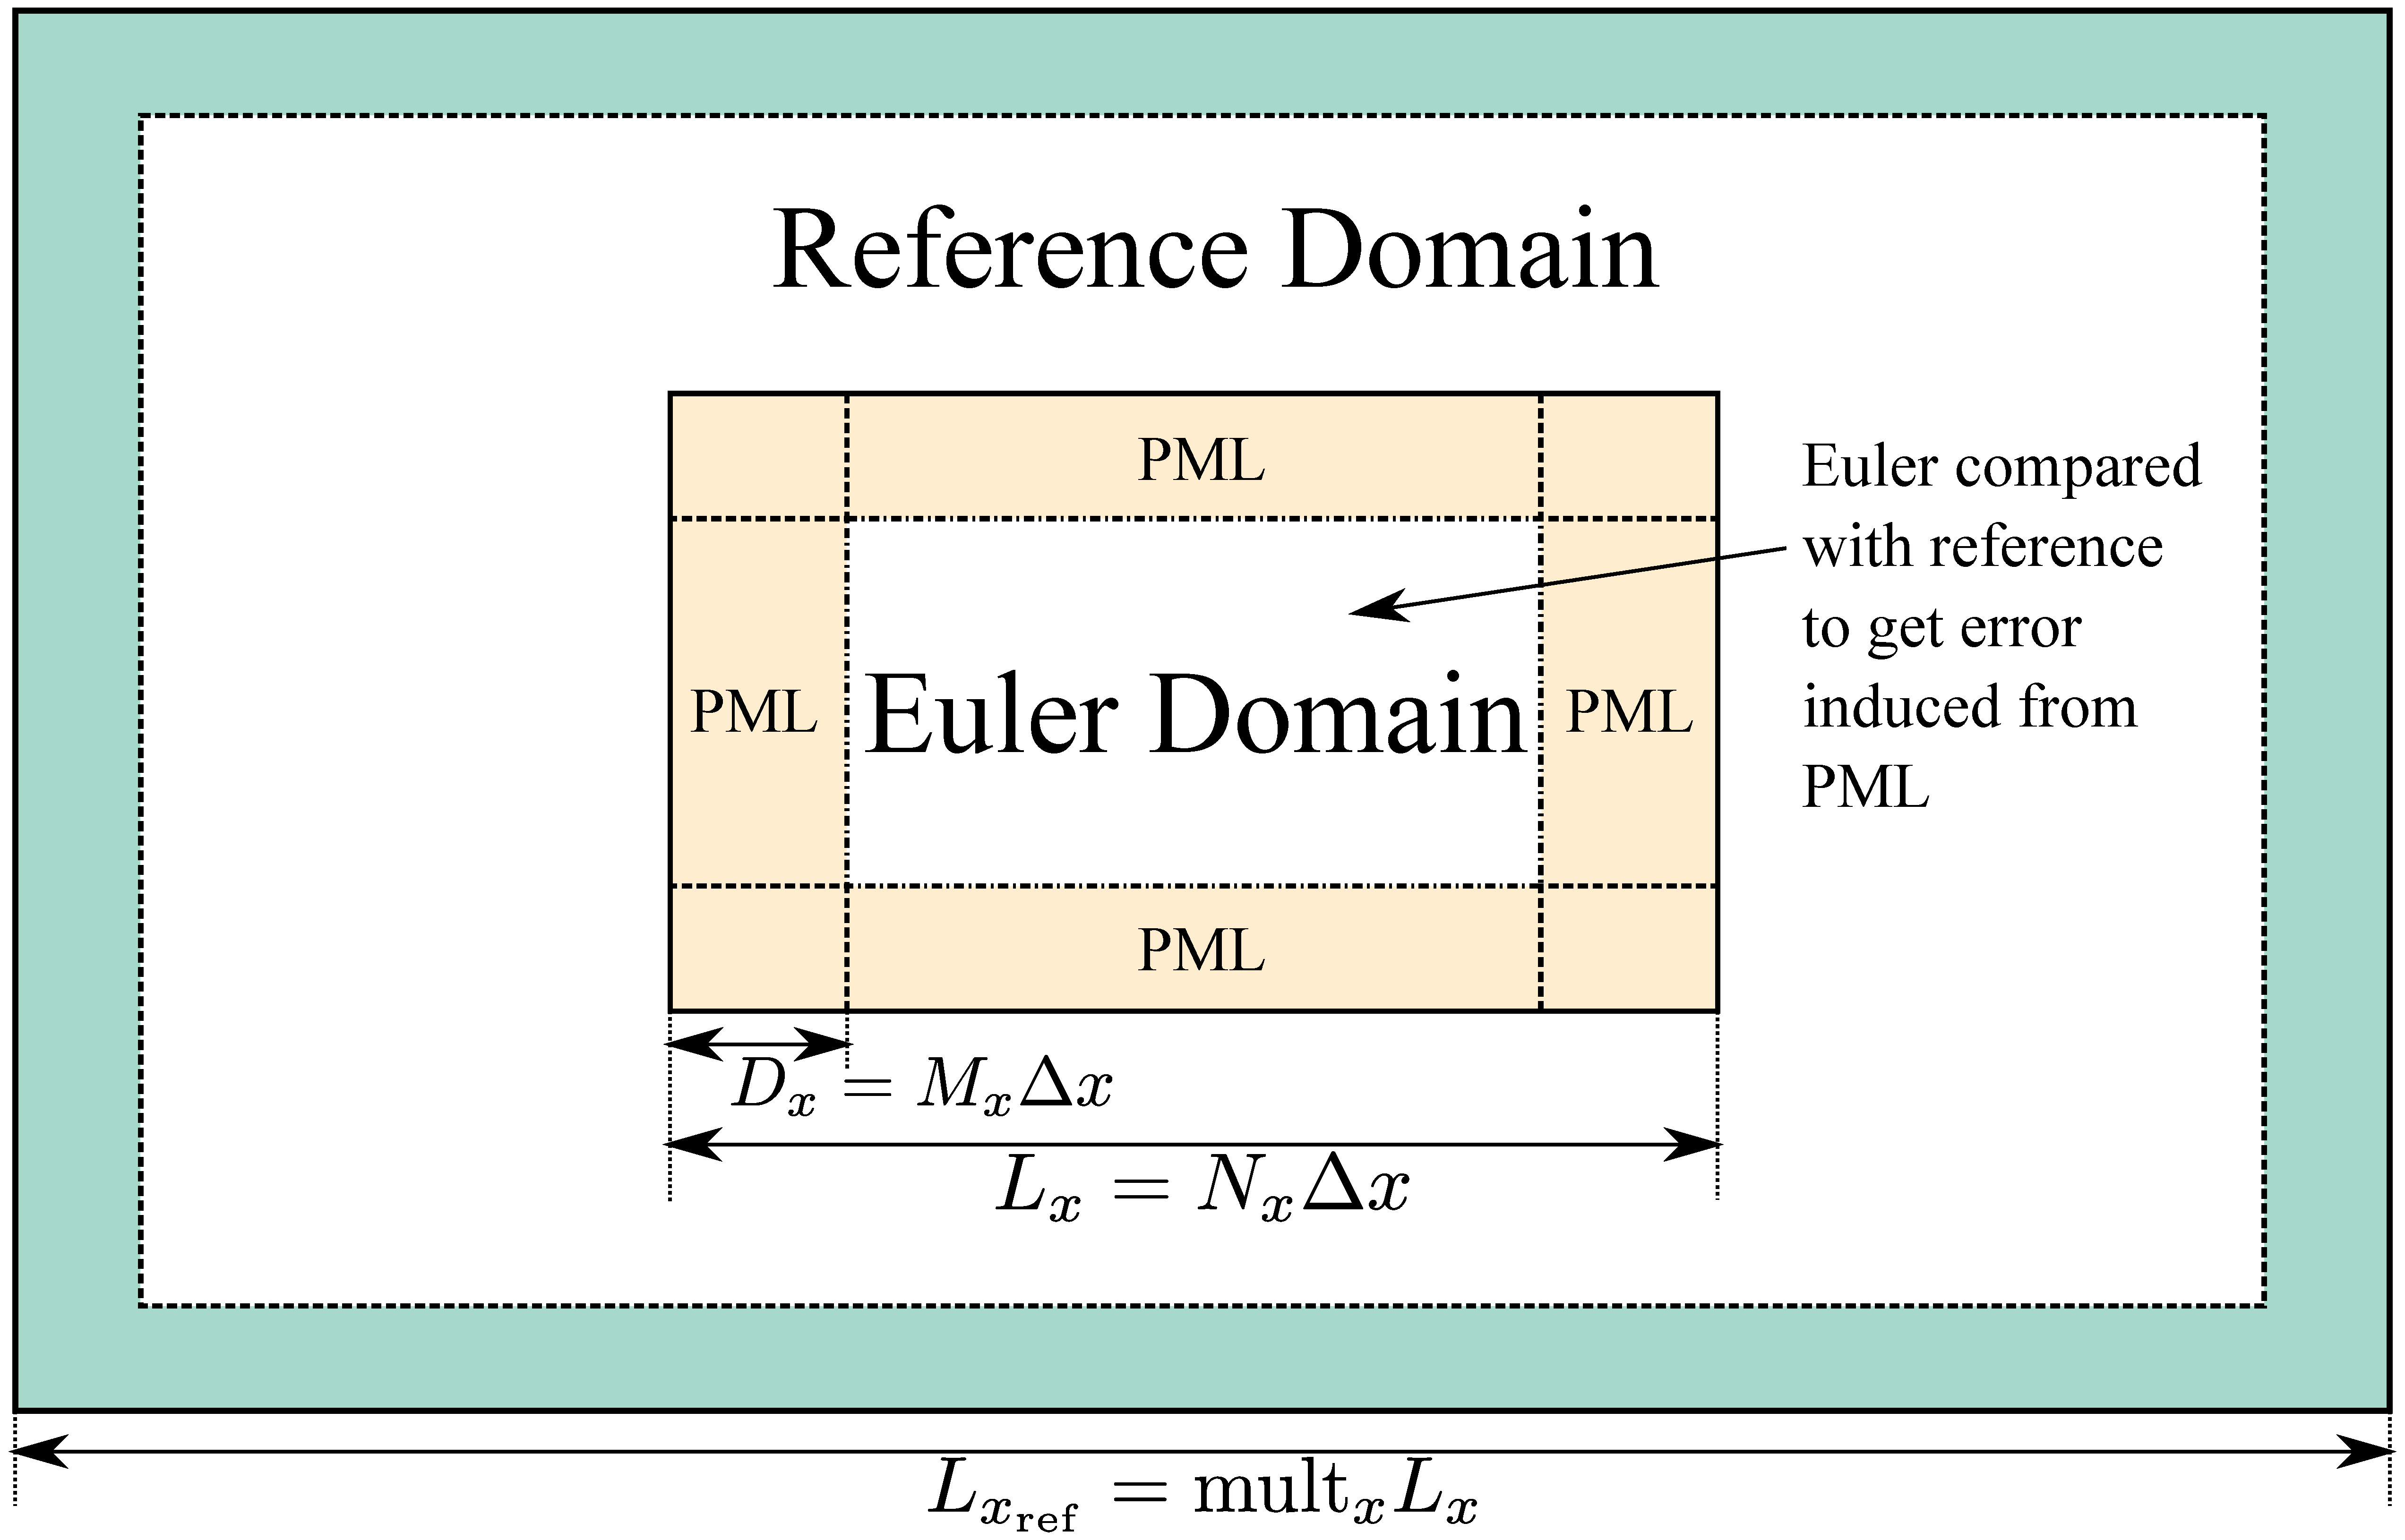
\includegraphics[width=12cm]{Figures/TechnicalAchievement/NumMeth/REFPMLDomain.eps}}
\caption{Euler and reference domain nomenclature. N.B. $y-$dimension variables follow similarly from $x-$dimension.}
\label{fig:REFPMLDomain}
\end{figure}